\chapter{Redes Neuronales Convolucionales}

Las redes neuronales convolucionales o CNN (\textit{Convolutional Neural Network}) son, en esencia, redes neuronales que emplen métodos convolucionales en vez de usar capas completamente conectadas. Las CNNs son increíblemente exitosas en su aplicación a problemas en los que los datos de entrada sobre los que se van a realizar predicciones tienen una topología conocida en forma de malla, como una serie temporal (que es una malla unidimensional) o una imagen (que es una malla bidimensional).

\section{Operacion Convolucional}

La operación convolucional en una dimensión consta de dos partes, un \textit{input} $I(t)$ y un \textit{kernel} $K(a)$, tal que la \textbf{operación convolucional} es 

\begin{equation}
    s(t) = \sum_a I(a) \cdot K(t-a)
\end{equation}
Una forma equivalente 
\begin{equation}
    s(t) = \sum_a I(t-a) \cdot K(a)
\end{equation}
En la literatura del aprendizaje máquina y su implementación en \textit{software}, la convolución y la correlación cruzada son intercambiables. La esencia de la operación es qeu el Kernel, mucho más pequeño que el input. El valor de la convolción $s(t)$ será, como tal, la salida de la operación convolucion. Evidentemente podemos generalizar este resultado para \textit{inputs} y \textit{kernels} de varias dimensiones, tales como

\begin{equation}
    s(m,n) = (I * K) (m,n) = \sum_{a} \sum_{b} I(a,b) \cdot K(m-a,n-b)
\end{equation}
Podemos pensar en la convolución como el producto de un vector/matriz pequeño sobre un área de un valor grande (input) centrado dando como resultado un único valor. Repetiremos este proceso sobre varias ``áreas'' del input obteniendo un output vector/matriz. 

En las imagenes \cref{Fig:04-CNN_Convolucional} y \cref{Fig:04-CNN_LayerDensity} podemos ver dos diferentes tipos de redes neuronales. En este caso es evidente ver que, para el mismo número de entradas y salidas, la densamente conectada tiene muchas mas conexiones (y por tanto más pesos) que la red convolucional. Debido a esto, lógicamente las interacciones que producen las salidas serán menores, o que llamamos red de interacción escasa o dispersa (\textit{sparse interaction}). Dado que los parámetros y pesos se comparten a lo largo de la capa convolucional, ya que se usa siempre el mismo kernel en la interacción de una capa a otra, pues tendremos muchos menos parámetros que en una red no convolucional. 

\begin{minipage}{0.45\linewidth} \centering
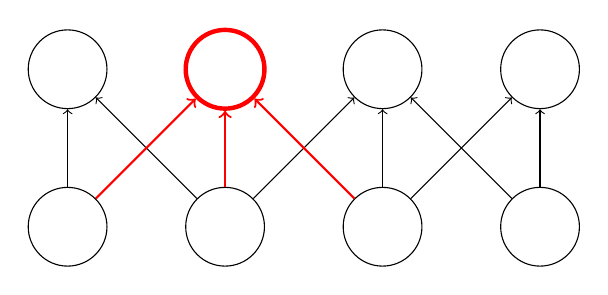
\begin{tikzpicture}

% Capa inferior
\node[circle, draw, minimum size=10mm] (I1) at (0,0) {};
\node[circle, draw, minimum size=10mm] (I2) at (2,0) {};
\node[circle, draw, minimum size=10mm] (I3) at (4,0) {};
\node[circle, draw, minimum size=10mm] (I4) at (6,0) {};

% Capa superior
\node[circle, draw, minimum size=10mm] (O1) at (0,2) {};
\node[circle, draw, minimum size=10mm, ultra thick, red] (O2) at (2,2) {};
\node[circle, draw, minimum size=10mm] (O3) at (4,2) {};
\node[circle, draw, minimum size=10mm] (O4) at (6,2) {};

% Conexiones negras
\draw[arrows={->}] (I1) -- (O1);
\draw[arrows={->}] (I2) -- (O1);
\draw[arrows={->}] (I2) -- (O3);
\draw[arrows={->}] (I3) -- (O3);
\draw[arrows={->}] (I3) -- (O4);
\draw[arrows={->}] (I4) -- (O3);
\draw[arrows={->}] (I4) -- (O4);

% Conexiones rojas hacia O2
\draw[arrows={->}, red, thick] (I1) -- (O2);
\draw[arrows={->}, red, thick] (I2) -- (O2);
\draw[arrows={->}, red, thick] (I3) -- (O2);

\end{tikzpicture}
\captionof{figure}{Red Neuronal Convolucional}
\label{Fig:04-CNN_Convolucional}
\end{minipage} \hfill
\begin{minipage}{0.45\linewidth} \centering
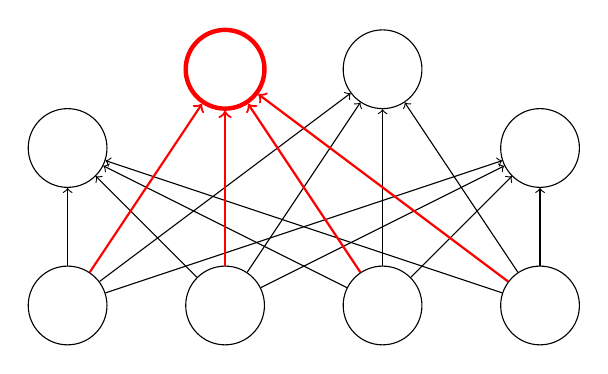
\begin{tikzpicture}

% Capa inferior
\node[circle, draw, minimum size=10mm] (I1) at (0,0) {};
\node[circle, draw, minimum size=10mm] (I2) at (2,0) {};
\node[circle, draw, minimum size=10mm] (I3) at (4,0) {};
\node[circle, draw, minimum size=10mm] (I4) at (6,0) {};

% Capa superior
\node[circle, draw, minimum size=10mm] (O1) at (0,2) {};
\node[circle, draw, minimum size=10mm, ultra thick, red] (O2) at (2,3) {};
\node[circle, draw, minimum size=10mm] (O3) at (4,3) {};
\node[circle, draw, minimum size=10mm] (O4) at (6,2) {};

% Conexiones negras
\draw[arrows={->}] (I1) -- (O1);
\draw[arrows={->}] (I1) -- (O3);
\draw[arrows={->}] (I1) -- (O4);

\draw[arrows={->}] (I2) -- (O1);
\draw[arrows={->}] (I2) -- (O3);
\draw[arrows={->}] (I2) -- (O4);

\draw[arrows={->}] (I3) -- (O1);
\draw[arrows={->}] (I3) -- (O3);
\draw[arrows={->}] (I3) -- (O4);

\draw[arrows={->}] (I4) -- (O1);
\draw[arrows={->}] (I4) -- (O3);
\draw[arrows={->}] (I4) -- (O4);

% Conexiones rojas hacia O2
\draw[arrows={->}, red, thick] (I1) -- (O2);
\draw[arrows={->}, red, thick] (I2) -- (O2);
\draw[arrows={->}, red, thick] (I3) -- (O2);
\draw[arrows={->}, red, thick] (I4) -- (O2);

\end{tikzpicture}
\captionof{figure}{Red Neuronal con capas densamente conmunicadas.}
\label{Fig:04-CNN_LayerDensity}
\end{minipage}

\section{Operacion de Agrupamiento}

\begin{minipage}{0.5\linewidth}
La \textbf{operación de Agrupamiento} o \textit{pooling operation} es una técnica que se usa junto con la convolución en las CNN. La idea detrás de la operación de \textit{pooling} es que la ubicación exacta de la característica no es un problema si, de hecho, esta ha sido detectada. Simplemente proporciona invariancia ante traslaciones. Por ejemplo, supongamos que la tarea en cuestión es aprender a detectar rostros en fotografías. Supongamos también que los rostros en la fotografía están inclinados (como generalmente ocurre) y que tenemos una capa de convolución que detecta los ojos. Nos gustaría abstraer la ubicación de los ojos en la fotografía de su orientación. La operación de pooling logra esto y es un componente importante de las CNN.

\vspace*{0.6em}

Lo que hacen estas operaciones es coger porciones de los \textit{inputs} y aplicarles la función $f$, produciendo una salida. Esta función $f$, normalmente una operación $\max$ (puede haber otras), actúa sobre porciones regulares (al menos en 2 dimensiones) 
\end{minipage} \hfill
\begin{minipage}{0.45\linewidth}
    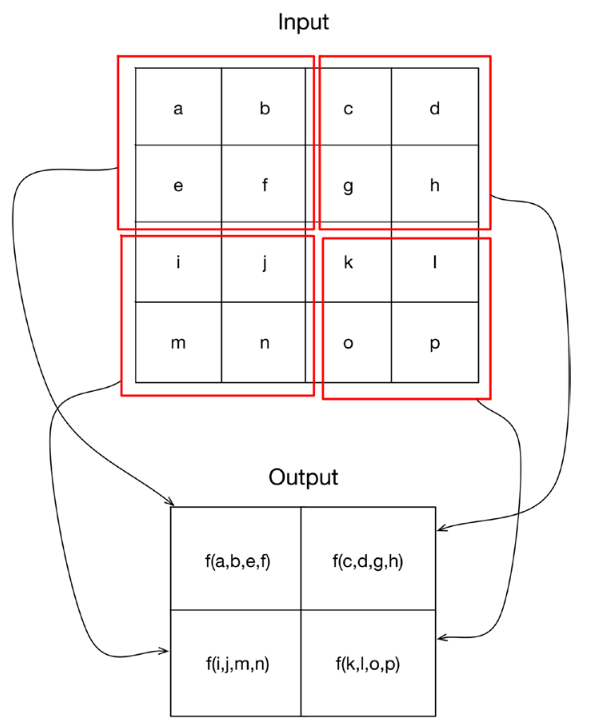
\includegraphics[width=1\linewidth]{Imagenes/04/Pooling.png}  
    \captionof{figure}{Ejemplo de una operación de Agrupamiento.} 
    \label{Fig:04-pooling}
\end{minipage}


y produce como resultado una salida dimensionalmente mucho más pequeña. En la \cref{Fig:04-pooling} representamos esta idea gráficamente. 

\section{Bloque básico de Convolución-Detector-Pooling}



\begin{minipage}{0.5\linewidth}
    
Ahora veremos como es un bloque básico en una red neuronal convolucional, donde mezclamos tanto procesos convolucionales como operaciones de agrupamiento. En la imagen \cref{Fig:04-pooling} vemos como una serie de inputs pasan a través de una red convolucional llegando pues a una capa o zona llamada detector (\textit{detector stage}) que es básicamente una función de activación no-lineal. La salida normalmente se pasa a otras capas (convolucionales o densamente conectadas). Lógicamente se pueden aplicar múltiples bloques de Convolución-Detector-Pooling en paralelo, utilizando la misma entrada y produciendo múltiples salidas o mapas de características (feature maps).

\end{minipage} \hfill
\begin{minipage}{0.45\linewidth}
    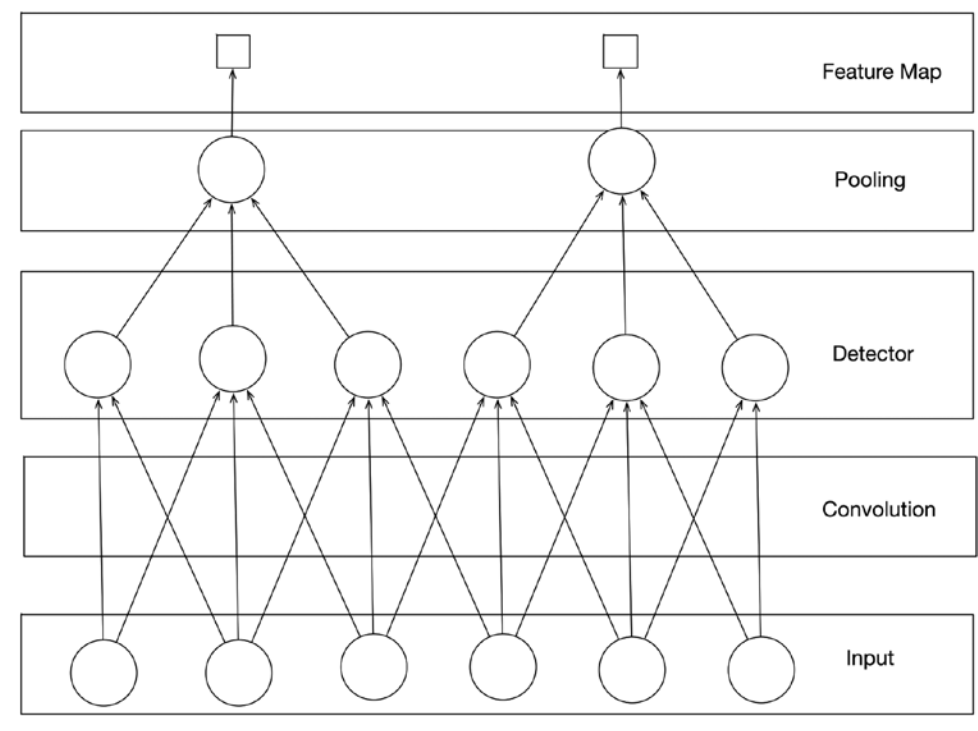
\includegraphics[width=1\linewidth]{Imagenes/04/PoolingBlock.png}  
    \captionof{figure}{Ejemplo de una operación de un bloque básico de detector-convolución-pooling.} 
    \label{Fig:04-poolingBlock}
\end{minipage}

\begin{minipage}{0.45\linewidth}
    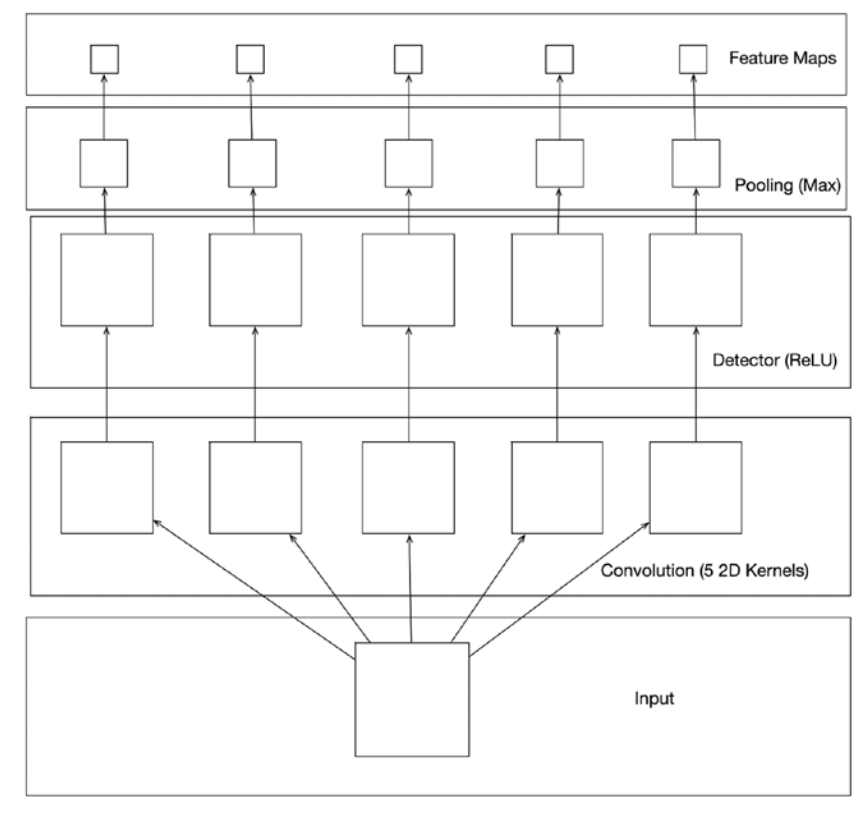
\includegraphics[width=1\linewidth]{Imagenes/04/PoolingFilter.png}  
    \captionof{figure}{Ejemplo de Kernels dando varias salidas.} 
    \label{Fig:04-poolingFilter}

\end{minipage} \hfill
\begin{minipage}{0.45\linewidth}
    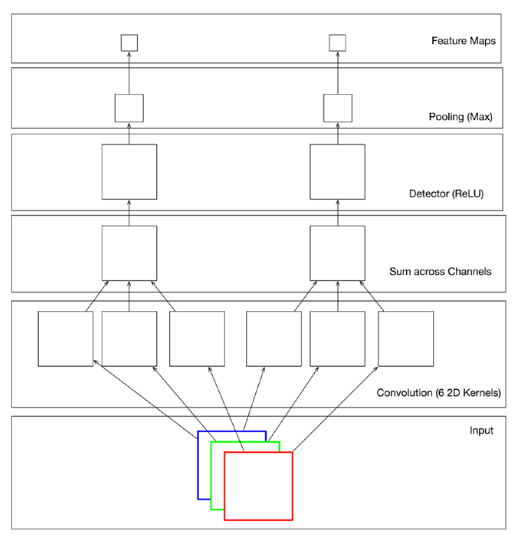
\includegraphics[width=1\linewidth]{Imagenes/04/PoolingMultiple.png}  
    \captionof{figure}{Convolución con varios canales.} 
    \label{Fig:04-poolingMultiple }
\end{minipage}

\section{Idea detrás de las redes neuronales convolucionales}

A lo largo de este capítulo hemos visto los conceptos básicos de las redes neuronales convolucionales, centrándonos en la operación convolución, la operación de agrupamiento o \textit{pooling} y como estas interactuan dentro de una CNN. Ahora bien, ¿Por qué se usan las CNNs? la primera idea que tenemos que considerar es su eficiencia. Las CNN, que en principio vienen a remplazar al menos una de las \textit{fully connected network}, en realidad tienen una pacaidad menor que estas, pero que a su vez, al tener menos parámetros únicos, deberían ser mucho más fáciles de entrenar (o al menos eficientemente). Otro de los aspectos a considerar vienen dados opr que, en realidad, los filtros manejados por la convolución, son capaces de detectar bordes, formas... Luego además debemos pensar en la operación agrupamiento, ya que esta en realidad nos permite separar el hecho de ser detectada una característica de la ubicación exacta de la característica (borde, forma...). Un filtro que detecta líneas rectas puede detectar este patrón en cualquier parte de la imagen, pero la operación de \textit{pooling} conserva el hecho de que la característica fue detectada (max \textit{pooling}). El útimo motivo es que la serie de capas de convolución y \textit{pooling} genera las características, y una red neuronal estándar aprende la función final de clasificación o regresión. Es importante distinguir este aspecto de las CNN del aprendizaje automático tradicional. En el aprendizaje automático tradicional, un experto diseñaba manualmente las características y las introducía en una red neuronal. En el caso de las CNN, estas características o representaciones se aprenden directamente a partir de los datos.